% !TeX spellcheck = lt
\documentclass{VUMIFPSbakalaurinis}
\usepackage{algorithmicx}
\usepackage{algorithm}
\usepackage{algpseudocode}
\usepackage{amsfonts}
\usepackage{amsmath}
\usepackage{bm}
\usepackage{caption}
\usepackage{color}
\usepackage{float}
\usepackage{graphicx}
\usepackage{listings}
\usepackage{subfig}
\usepackage{url}
\usepackage{wrapfig}
\usepackage[table,xcdraw]{xcolor}
\usepackage[backend=biber]{biblatex}
\usepackage{enumitem}\setlist{nosep}
\usepackage{csquotes}
\usepackage{setspace}
\usepackage[colorlinks=false]{hyperref} 

%\onehalfspacing

% Titulinio aprašas
\university{Vilniaus universitetas}
\faculty{Informatikos institutas}
\department{Programų sistemos}
%\papertype{Bakalauro darbas}
\papertype{Bakalauro baigiamasis darbas}
%Skatinamojo mokymosi algoritmu skirtu Sokoban zaidimo agento valdymui palyginimas
\title{Skatinamojo mokymosi taikymas žaidimo agento valdymo programos kūrimui}
\titleineng{Application of reinforcement learning to the software development for game agent management}
\author{Jokūbas Rusakevičius}
\supervisor{vyresn. m.d. Virginijus Marcinkevičius}
\reviewer{j. asist. Linas Petkevičius}
\date{Vilnius – \the\year}

\setmainfont{Palemonas}
\bibliography{bibliografija}

\begin{document}
\maketitle
\setcounter{page}{2}

\sectionnonumnocontent{}
\vspace{7cm}
\begin{center}
Dėkoju šeimai ir draugams, už meilę ir nuolatinį palaikymą bei darbo vadovui, vyresn. m.d. Virginijui Marcinkevičiui, už visapusišką pagalbą geriausio sprendimo beieškant.
\end{center}


\sectionnonumnocontent{Santrauka}
TODO: Santrauka
% Nurodomi iki 5 svarbiausių temos raktinių žodžių (terminų).
% Vienas terminas gali susidėti iš kelių žodžių.
\raktiniaizodziai{Skatinamasis mokymas, Sokoban žaidimas, aktorius-kritikas based metodai, raktinis žodis 4, raktinis žodis 5}   

\sectionnonumnocontent{Summary}
TODO: summary
\keywords{Reinforcement learning, Sokoban game, actor-critic based methods, keyword 4, keyword 5}

\tableofcontents

\sectionnonum{Įvadas}\label{sec:ivadas}
\subsectionnonum{Problematika}\label{subsec:problematika}
Kompiuterių pajėgumui ir atliekamų operacijų per sekundę skaičiui nuolatos didėjant -- didėja ir lūkesčiai bei sprendžiamų uždavinių sudėtingumas. Dar reliatyviai neseniai sudėtingiausios programos ir kompiuterių sprendžiami uždaviniai susidėjo iš skaičiuotuvo operacijų ar žinučių perdavimo. Tačiau technologijoms tobulėjant, kiekvienam žmogui kišenėje besinešiojant pirmųjų kompiuterių kaip \enquote{ENIAC} \cite{computer_history} dydį pajuokiančius kompiuterinius įrenginius, natūraliai didėja ir jiems keliami iššūkiai.\par

Šiais laikais kompiuteriai gali simuliuoti atominius sprogimus, nuspėti orus ir atlikti kitas didžiulių skaičiavimo išteklių reikalaujančias užduotis \cite{supercomputers}. Tačiau užduoties sudėtingumą gali lemti ne tik milžiniškų išteklių skaičiaus reikalavimas. 2016 metais matėme, kaip \enquote{Google’s AlphaGo} nugalėjo pasaulio aukščiausio lygio \enquote{Go} žaidėją ir čempioną Ke Jie \cite{go}. Autonominiai gatvėmis važinėjantys automobiliai neišvengiamai artėja, o \enquote{Boston Dynamics} robotai stebina savo galimybėmis \cite{bostondynamics}.\par

Šie uždaviniai nėra trivialiai aprašomi ar išsprendžiami, jiems gali net neegzistuoti sprendimas. Tokiems uždaviniams spręsti yra naudojami mašininio mokymosi metodai (pvz. neuroniniai tinklai). Viena šių metodų šaka yra \enquote{skatinamasis mokymas} -- agento atliekami veiksmai yra reguliariai vertinami ir atitinkamai agentas yra apdovanojamas arba baudžiamas.

..Kažką apie sokoban...


\subsectionnonum{Darbo tikslas}\label{subsec:tikslas}
Šio darbo \textbf{tikslas} -- išanalizavus populiariausius skatinamojo mokymosi algoritmus, pritaikyti kelis labiausiai tinkamus Sokoban žaidimo aplinkai.......

\subsectionnonum{Darbo uždaviniai}\label{subsec:uzdaviniai}
Darbui iškelti \textbf{uždainiai}:
\begin{enumerate}
	\item Paruošti eksperimentinę aplinką ir agentą.
	\item
\end{enumerate}

\section{Teorija}\label{sec:1}


\subsection{Skatinamasis mokymasis}\label{subsec:RL} 
{
	Skatinamasis mokymasis (RL), kartu su prižiūrimuoju ir neprižiūrimuoju mokymu, yra viena iš pagrindinių mašinų mokymosi (ML) paradigmų. Klasikinis RL modelis susideda iš agento (\textit{angl. agent}), kuris priima sprendimus ir atlieka veiksmus (\textit{angl. actions}) pagal strategiją  (\textit{angl. policy}), paremtus aplinkos būsena (\textit{angl. state}), ir siekiantis pasiekti didžiausią įmanomą atlygį (\textit{angl. reward}).\par
	
	Skirtingai nei kitos ML paradigmos, RL sprendžia ne regresijos, klasifikacijos, ar grupavimo, bet atlygiu paremtas (\textit{angl. reward-based}) problemas, ir tai daro bandymų ir klaidų (\textit{ang. trial and error}) principu. Dėmesys yra nukreiptas ne į sužymėtas (\enquote{angl. labeled}) įvesties ir išvesties duomenų poras, bet į balanso tarp tyrinėjimo (\textit{angl. exploration}) ir išnaudojimo (\textit{angl. exploitation}) ieškojimą \cite{kaelbling_littman_moore}.\par
	
	RL algoritmai yra skirstomi pagal skirtingus rodiklius į kelias skirtingas kategorijas. Prieš aiškinantis kuo skiriasi kiekviena kategorija, svarbu suprasti, kad RL algoritmai susideda iš dviejų fazių:
	
	\begin{enumerate}
		\item \textbf{Mokymosi fazė} -- (\textit{angl. learning phase}) tai yra algoritmo apmokymo dalis, kai kiekvienas agento priimtas sprendimas ir atliktas veiksmas aplinkoje bei gautas atlygis ir nauja aplinkos būsena yra panaudojama tolimesniam modelio optimizavimui ir gerinimui.
		\item \textbf{Taikymo fazė} -- (\textit{angl. interface phase}) tai yra algoritmo dalis, kai, nepriklausomai nuo atlikto veiksmo optimalumo, modelis nebėra keičiamas ir yra naudojamos iki šiol išmoktos reikšmės.
	\end{enumerate}

	 Kaip jau minėta anksčiau, RL algoritmai yra skirstomi į skirtingas kategorijas. Pagal modelio struktūrą:
	 
	\begin{enumerate}
		\item \textbf{Pagrįsti modeliu} -- (\textit{angl. model-based}) tai yra algoritmai, kurie optimalios strategijos apskaičiavimui naudojasi transakcijų funkcija (ir atlygio funkcija) (daugiau poskyryje~\ref{subsubsec:MDP}). Pagrįsti modeliu algoritmai gali nuspėti galimus aplinkos pakitimus, kadangi naudojasi apskaičiuota transakcijų funkcija. Tačiau, modelio turima funkcija gali būti tik apytikslė \enquote{tikrajai} funkcijai, tad modelis gali niekada nepasiekti optimalaus sprendimo. 
		\item \textbf{Nepagrįsti modeliu} -- (\textit{angl. model-free}) tai yra algoritmai, kurie apskaičiuodami optimalią strategija nesinaudoja ir nebando apskaičiuoti aplinkos dinamikų (transakcijų ir perėjimų funkcijos nenaudojamos). Nepagrįsti modeliu algoritmai bando apskaičiuoti vertės arba strategijos funkciją tiesiai iš patirties (interakcijų su aplinka).
	\end{enumerate}

	Pagal strategijos pritaikymą:
	
	\begin{enumerate}
		\item \textbf{Besiremiantys optimalia strategija} -- (\textit{angl. on-policy}) algoritmai, kurie, mokymosi metu rinkdamiesi veiksmą, remiasi strategija išvesta iš tuo metu apskaičiuotos optimaliausios strategijos bei atlieka atnaujinimus remdamiesi ta pačia strategija.
		\item \textbf{Nesiremiantys optimalia strategija} -- (\textit{angl. off-policy}) algoritmai, kurie mokymosi metu remiasi skirtinga strategija nei tuo metu apskaičiuota optimaliausia strategija. Atnaujinimai atliekami remiantis geresnį rezultatą gražinančia strategija.
	\end{enumerate}

	Pagal ... asasdasd~\ref{subsubsec:MDP}:
	
	\begin{enumerate}
		\item \textbf{Pagrįsti verte} -- (\textit{angl. value-based}) tai yra algoritmai pagrįsti \textit{laiko skirtumų mokymusi} (\textit{angl. temporal difference learning}), kur yra mokomasi funkcija \(V^{\pi}\)  arba \(V^*\) (daugiau poskyryje~\ref{subsubsec:rlTeorija}).
		\item \textbf{Pagrįsti strategija} -- (\textit{angl. policy-based}) tai algoritmai, kurie tiesiogiai mokosi optimalios strategijos \(\pi^*\) arba bando apytiksliai surasti optimalią strategiją.
	\end{enumerate}

	Toliau šiame poskyryje bus giliau nagrinėjamas RL ir jį sudarantys elementai.
}

\subsubsection{Skatinamojo mokymosi teorija} \label{subsubsec:rlTeorija} 
{
	Šiame darbe bus remiamasi standartine RL aplinka, kur agentas yra aplinkoje \(\mathcal{E}\) diskretų kiekį laiko vienetų arba žingsnių (\textit{angl. time steps}). Kiekvieną žingsnį \(t\) agentas gauna informaciją apie aplinkos būseną \(s_t\) ir iš visų įmanomų veiksmų rinkinio \(\mathcal{A}\) pasirenka atitinkamą veiksmą \(a_t\) pagal strategiją \(\pi\), kur \(\pi\) yra sužymėjimas kokį veiksmą \(a_t\) rinktis situacijoje \(s_t\). Aplinka agentui grąžina informaciją apie sekančią aplinkos būseną \(s_{t+1}\) ir skaliarinę atlygio reikšmę \(r_t\). Toks procesas yra tęsiamas, kol aplinka pasiekia galinę būseną (\textit{angl. terminal state}). Kai galinė būsena yra pasiekiama -- procesas yra pradedamas iš naujo. Rezultatas \(R_t = \sum_{k=0}^{\infty} \gamma^k r_{t+k}\) yra bendras žingsnyje \(t\) surinktas atlygis su nuolaidos koeficientu (\textit{angl. discount factor}) \(\gamma \in (0, 1] \). Agento tikslas yra gauti didžiausia įmanoma tikėtina rezultatą iš visų aplinkos būsenų \(s_t\).\par
	
	Veiksmo vertė (\textit{angl. value}) apskaičiuojama: \(Q^{\pi}(s, a) = \mathbb{E}[R_t|s_t = s, a] \), kur tikėtinas rezultatas \(\mathbb{E}\) gaunamas pagal strategiją \(\pi\) pasirinkus veiksmą \(a\), esant situacijoje \(s\). Optimali vertės funkcija \(Q^*(s, a) = \max_{\pi}Q^{\pi}(s, a)\), grąžina didžiausią strategijos \(\pi\) pasiektą veiksmo vertę aplinkos būsenai \(s\) ir veiksmui \(a\). Panašiai, aplinkos būsenos \(s\) vertė remiantis strategija \(\pi\) yra apibrėžiama taip: \(V^{\pi}(s) = \mathbb{E}[R_t|s_t = s] \), ir yra tikėtinas rezultatas būsenai \(s\) pagal strategiją \(\pi \).\par

}

\subsubsection{Gilusis mokymas}
\subsubsection{Markovo procesas}\label{subsubsec:MDP}
{ 
	Pirmieji aprašyti Markovo procesai (MDP) \cite{mdp} priminė Markovo grandines (\textit{angl. Markov chains}).\par
	
	\textbf{Markovo grandinė} -- tai kiekviename žingsnyje atsitiktinai judantis iš vienos į kitą būseną (\textit{angl. state}) procesas su fiksuotu skaičiumi būsenų, kur tikimybė pereiti iš būsenos \(s\) į būseną \(s'\) yra taip pat fiksuota ir priklauso tik nuo poros \((s, s')\), ne nuo jau praėjusių būsenų. Markovo grandinės neturi atminties \cite{handson}. 
	
	\begin{figure}[H]
		\centering
		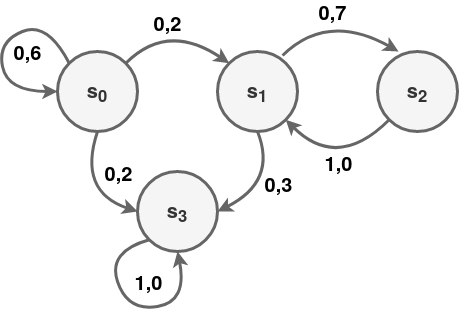
\includegraphics[scale=0.5]{img/markov_chain}
		\caption{Markovo grandinės pavyzdys}
		\label{img:markovChain}
	\end{figure} 
	
	Paveikslėlyje~\ref{img:markovChain} pavaizduotas Markovo grandinės pavyzdys su keturiomis būsenomis. Jeigu laikome būseną \(s_0\) pradine, tai yra \(60\%\) tikimybė, kad procesas pasiliks šioje būsenoje ir kitą žingsnį. Po tam tikro kiekio žingsnių, procesas galiausiai paliks \(s_0\) ir niekada nebegrįš į šią būseną, nes jokia kita rodyklė nerodo į \(s_0\). Jei procesas pereis į būseną \(s_1\), tai yra labiausiai tikėtina (\(60\%\) tikimybė), jog kita būsena bus \(s_2\)) ir tada iškart atgal į \(s_1\) (\(100\%\) tikimybė). Procesas gali pereiti per \(s_1\) \(s_2\) kelis kartus, prieš galiausiai patenkant į galinę būseną \(s_3\), kur procesas ir pasiliks.\par
	
	MDP nuo Markovo grandinės skiriasi tuo, kad MDP perėjimai iš vienos būsenos į kitą, gali turėti jiems priskirtus atlygius (gali būti teigiami ir neigiami). RL problemos labai dažnai yra formuluojamos kaip MDP, kur agento tikslas yra surasti strategija, kuri privestų prie didžiausio bendro atlygio per trumpiausia laiko tarpą \cite{handson}.\par
	
	\begin{figure}[H]
		\centering
		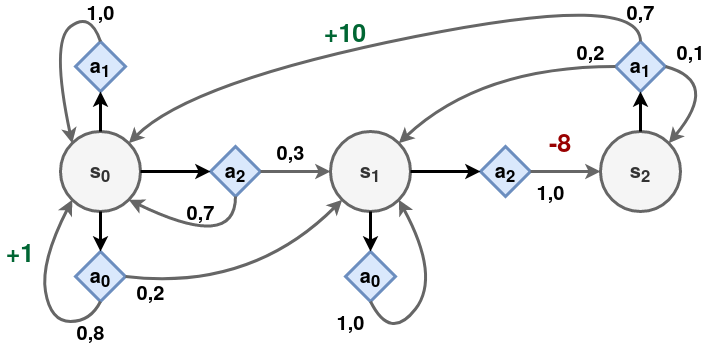
\includegraphics[scale=0.5]{img/mdp}
		\caption{Markovo proceso pavyzdys}
		\label{img:mdp}
	\end{figure} 
	
	Paveikslėlyje~\ref{img:mdp} pavaizduotas MDP pavyzdys su trimis būsenomis ir iki trijų diskrečių veiksmų per būseną. Jeigu laikome, kad agentas pradeda būsenoje \(s_0\), tai pirmame žingsnyje agentas gali pasirinkti vieną iš trijų galimų: \(a_0\), \(a_1\), \(a_2\) veiksmų. Jeigu agentas pasirinktų atlikti veiksmą \(a_1\) -- jis garantuotai liktų būsenoje \(s_0\). Tačiau, jeigu agentas pasirinktų veiksmą \(a_0\) -- yra \(80\%\) tikimybė, gauti atlygį \(+1\) ir likti toje pačioje būsenoje \(s_0\) arba \(20\%\) tikimybė be atlygio patekti į būseną \(s_1\). Galiausiai arba \(a_0\), arba \(a_2\) veiksmu agentas pateiks į būseną \(s_1\). Šioje būsenoje agentas gali pasirinkti tik vieną iš dviejų veiksmų: \(a_0\) arba \(a_2\). Nors yra du galimi veiksmai, tik veiksmas \(a_2\) veda į kitą būseną. Tačiau pasirinktus šį veiksmą agentas taip pat garantuotai gauna atlygį (bausmę) \(-8\). Pasiekus būseną \(s_3\) yra galimas tik vienas veiksmas \(a_1\), bet galimi trys skirtingi rezultatai: likti toje pačioje būsenoje \(s_3\) (\(10\%\) tikimybė), pereiti į būseną \(s_1\) (\(20\%\) tikimybė) arba grįžti į pradinę būseną \(s_0\) (\(70\%\) tikimybė) ir gauti atlygį \(+10\).\par
	
	Optimaliai būsenos vertei bet kuriai būsenai \(s\), žymimai \(V^*(s)\), nustatyti, galima naudoti \textit{Belmano Optimalumo Lygtį}. Ši rekursyvi lygtis~\ref{eq:bellmanOptimal} parodo, kad jei agentas atlieka veiksmus optimaliai, tada optimali dabartinės būsenos reikšmė yra lygi vidutiniškai agento gaunamam atlygiui atlikus vieną optimalų veiksmą, plius visų įmanomų toliau einančių būsenų tikėtina optimali vertė.
	
	\begin{equation}\label{eq:bellmanOptimal}
		V^* = \max_a \Sigma_{s'}T(s, a, s')[R(s, a, s') + \gamma V^*(s')] \textrm{ su visais } s
	\end{equation} 
	
	\begin{itemize}
		\item \textbf{Transakcijų funkcija} (\textit{angl. transaction function}) \(T(s, a, s')\) yra perėjimo iš būsenos \(s\) į būseną \(s'\) tikimybė, agentui pasirinkus veiksmą \(a\).
		\item \textbf{Atlygio funkcija} (\textit{angl. reward function}) \(R(s, a, s')\) yra agento gaunamas atlygis, kai jis pereina iš būsenos \(s\) į būseną \(s'\), agentui pasirinkus veiksmą \(a\).
		\item \(\gamma\) yra nuolaidos koeficientas.
	\end{itemize}

	MDP taip pat gali būti užrašyta taip: \(\mathcal{M} = (\mathcal{S}, \mathcal{A}, P, R, \gamma)\).
	\begin{itemize}
		\item \(\mathcal{S}\): visų būsenų rinkinys.
		\item \(\mathcal{A}\): visų veiksmų rinkinys.
		\item \(P : \mathcal{S} \times \mathcal{A} \times \mathcal{S} \rightarrow [0, 1]\): transakcijų tikimybės pasiskirstymas \(P(s'|s, a)\).
		\item \(R : \mathcal{S} \rightarrow \mathbb{R}\): atlygio funkcija, \(R(s)\) yra atlygis būsenai \(s\).
		\item \(\gamma\): nuolaidos koeficientas.
	\end{itemize}
}
\subsubsection{Sustiprinto mokymosi strategijos ieškojimas}
\subsubsubsection{MlpPolicy}
\subsubsubsection{CnnPolicy}
\subsubsubsection{LSTM}
\subsubsection{Aktoriaus-kritiko principas}

\subsection{Neuroniniai tinklai}
\subsubsubsection{Gilieji neuroniniai tinklai}
\subsubsubsection{Konvoliuciniai neuroniniai tinklai}



\section{Metodologija}
\subsection{Sokoban žaidimas}
\subsubsection{OpenAI Gym}

\subsection{Skatinamojo mokymosi bibliotekos parinkimas}
\subsubsection{Stable Baselines architektūra}
\subsubsubsection{A2C aprašymas}
\subsubsubsection{ACER aprašymas}
\subsubsubsection{POP2 aprašymas}

\section{Eksperimentai}
Šiame skyriuje aprašomi bakalauro darbo metu atlikti eksperimentai bei jiems paruošta eksperimentinė aplinka.

\subsection{Sokoban aplinkos paruošimas}
Šiame poskyryje yra aprašomas metodas eksperimento metu tiriamos Sokoban aplinkos paruošimui.
\subsubsection{}


\subsection{Eksperimentinė aplinka}
Eksperimentai atlikti naudojantis realia mašina su \enquote{Ubuntu} OS. Minėtoje mašinoje įdiegta \enquote{Anaconda} paketų valdymo ir dislokavimo sistema, naudojama aplinkų atskyrimui. Didžioji programinė dalis eksperimento atliekama \enquote{Jupyter Notebook} programavimo aplinkoje naudojantis \enquote{Python} kalba.

\subsubsection{Eksperimentinės aplinkos specifikacijos}
Eksperimentas atliekamas naudojantis realią \enquote{Ubuntu} mašiną.

\begin{enumerate}
	\item Kompiuterio techninė specifikacija:
	\begin{enumerate}
		\item Procesorius -- \enquote{\textbf{Intel Core i5-9600K}} (6 branduoliai, bazinis greitis 3.70 GHz).
		\item Grafinė vaizdo plokštė -- \enquote{\textbf{Nvidia GeForce RTX 2070 Super}}.
		\item Operatyvioji atmintis -- \enquote{\textbf{HyperX Predator Black}} (\textbf{32GB}, 3200MHz, DDR4, CL16).
		\item Pastovioji atmintis -- \enquote{\textbf{Western Digital}} (\textbf{1TB}).
	\end{enumerate}

	\item Kompiuterio programinė įranga:
	\begin{enumerate}
		\item Operacinė sistema -- \enquote{\textbf{Ubuntu 18.04 LTS}} (versija: \textbf{18.04.4 LTS}).
		\item Paketų ir aplinkų valdymo sistema - \enquote{\textbf{Anaconda}}  (versija: \textbf{2020.02}).
		\item Programavimo kalba -- \enquote{\textbf{Python}} (versija: \textbf{3.7.6}).
		\item Atviro kodo programa kintančio kodo, matematinių funkcijų, teksto bei duomenų vizualizavimui -- \enquote{\textbf{Jupyter Notebook}}  (versija: \textbf{6.0.3}).
		\item ... -- \enquote{\textbf{Tensorflow}} (versija: \textbf{1.14.0}).
		\item ... -- \enquote{\textbf{OpenAI Gym}} (versija: \textbf{0.17.1}).
		\item ... -- \enquote{\textbf{Stable Baselines}} (versija: \textbf{2.10.1a0}).
		\item Išskirstyta VSC sistema pakeitimų sekimui kode -- \enquote{\textbf{Git}} (versija: \textbf{2.23.0}) 
	\end{enumerate}
\end{enumerate}

\subsubsection{Ekseperimentinės aplinkos paruošimas}

\subsection{Eksperimento planas}
Darbo metu atliktas eksperimentas susideda iš trijų dalių. Šiame skyriuje yra aprašomi šių trijų eksperimentų planai: kaip bus atliekamas eksperimentas, kokia bus naudojama aplinka, kokių rezultatų yra tikimasi ir pan.
\subsubsubsection{Pirmo eksperimento planas: Geriausios strategijos ieškojimas}


\subsubsection{Eksperimentas}

\printbibliography[heading=bibintoc] 

\sectionnonum{Santrumpos}
Darbe naudojamų santrumpų paaiškinimai:
\begin{itemize}[label={}] %, leftmargin=*] %apgalvoti kaip padaryti šį sąrašą
	\item \textbf{A2C} -- (\textit{angl. Advantage Actor-Critic}) ...
	\item \textbf{ACER} -- (\textit{angl. Actor-Critic with Experience Replay}) ...
	\item \textbf{MDP} -- (\textit{angl. Markov Decision Processes}) Markovo procesas.
	\item \textbf{ML} -- (\textit{angl. Machine Learning}) mašinų (arba kompiuterių) mokymasis.
	\item \textbf{PPO2} -- (\textit{angl. Proximal Policy Optimization}) ...
	\item \textbf{RL} -- (\textit{angl. Reinforcement Learning}) skatinamasis mokymas.
	\item \textbf{VSC} -- (\textit{angl. Version-Control System}) versijų tvarkymo sistema.
\end{itemize}

%\appendix

\section{a}

\end{document}
